\PassOptionsToPackage{unicode=true}{hyperref} % options for packages loaded elsewhere
\PassOptionsToPackage{hyphens}{url}
%
\documentclass[11pt,ignorenonframetext,]{beamer}
\usepackage{pgfpages}
\setbeamertemplate{caption}[numbered]
\setbeamertemplate{caption label separator}{: }
\setbeamercolor{caption name}{fg=normal text.fg}
\beamertemplatenavigationsymbolsempty
% Prevent slide breaks in the middle of a paragraph:
\widowpenalties 1 10000
\raggedbottom
\setbeamertemplate{part page}{
\centering
\begin{beamercolorbox}[sep=16pt,center]{part title}
  \usebeamerfont{part title}\insertpart\par
\end{beamercolorbox}
}
\setbeamertemplate{section page}{
\centering
\begin{beamercolorbox}[sep=12pt,center]{part title}
  \usebeamerfont{section title}\insertsection\par
\end{beamercolorbox}
}
\setbeamertemplate{subsection page}{
\centering
\begin{beamercolorbox}[sep=8pt,center]{part title}
  \usebeamerfont{subsection title}\insertsubsection\par
\end{beamercolorbox}
}
\AtBeginPart{
  \frame{\partpage}
}
\AtBeginSection{
  \ifbibliography
  \else
    \frame{\sectionpage}
  \fi
}
\AtBeginSubsection{
  \frame{\subsectionpage}
}
\usepackage{lmodern}
\usepackage{amssymb,amsmath}
\usepackage{ifxetex,ifluatex}
\usepackage{fixltx2e} % provides \textsubscript
\ifnum 0\ifxetex 1\fi\ifluatex 1\fi=0 % if pdftex
  \usepackage[T1]{fontenc}
  \usepackage[utf8]{inputenc}
  \usepackage{textcomp} % provides euro and other symbols
\else % if luatex or xelatex
  \usepackage{unicode-math}
  \defaultfontfeatures{Ligatures=TeX,Scale=MatchLowercase}
\fi
\usetheme[]{Montpellier}
\usecolortheme{beaver}
% use upquote if available, for straight quotes in verbatim environments
\IfFileExists{upquote.sty}{\usepackage{upquote}}{}
% use microtype if available
\IfFileExists{microtype.sty}{%
\usepackage[]{microtype}
\UseMicrotypeSet[protrusion]{basicmath} % disable protrusion for tt fonts
}{}
\IfFileExists{parskip.sty}{%
\usepackage{parskip}
}{% else
\setlength{\parindent}{0pt}
\setlength{\parskip}{6pt plus 2pt minus 1pt}
}
\usepackage{hyperref}
\hypersetup{
            pdftitle={Etude des effets des pésticides dans la production des vins de table},
            pdfauthor={A. Blanc, N. Gusarov, S. Picon},
            pdfborder={0 0 0},
            breaklinks=true}
\urlstyle{same}  % don't use monospace font for urls
\newif\ifbibliography
\usepackage{graphicx,grffile}
\makeatletter
\def\maxwidth{\ifdim\Gin@nat@width>\linewidth\linewidth\else\Gin@nat@width\fi}
\def\maxheight{\ifdim\Gin@nat@height>\textheight\textheight\else\Gin@nat@height\fi}
\makeatother
% Scale images if necessary, so that they will not overflow the page
% margins by default, and it is still possible to overwrite the defaults
% using explicit options in \includegraphics[width, height, ...]{}
\setkeys{Gin}{width=\maxwidth,height=\maxheight,keepaspectratio}
\setlength{\emergencystretch}{3em}  % prevent overfull lines
\providecommand{\tightlist}{%
  \setlength{\itemsep}{0pt}\setlength{\parskip}{0pt}}
\setcounter{secnumdepth}{0}

% set default figure placement to htbp
\makeatletter
\def\fps@figure{htbp}
\makeatother

\usepackage{array}
\usepackage{multicol}

\title{Etude des effets des pésticides dans la production des vins de table}
\providecommand{\subtitle}[1]{}
\subtitle{Analyse empirique des marchés}
\author{A. Blanc, N. Gusarov, S. Picon}
\providecommand{\institute}[1]{}
\institute{Université Grenoble Alpes}
\date{11/12/2019}

\begin{document}
\frame{\titlepage}

\begin{frame}
\tableofcontents[hideallsubsections]
\end{frame}
\begin{frame}{Introduction}
\protect\hypertarget{introduction}{}

Dans cet étude, nous chercherons à étudier l'équilibre sur le marché du
vin.

Nous chercherons à répondre à la question suivante :

\begin{itemize}
\tightlist
\item
  Quel est l'effet de la demande de pesticide sur l'équilibre des vins
  simples ?
\end{itemize}

\end{frame}

\begin{frame}{Plan de la présentation}
\protect\hypertarget{plan-de-la-presentation}{}

\begin{itemize}
\tightlist
\item
  Présentation de la problématique
\item
  Présentation des données
\item
  Modélisation
\item
  Les résultats
\end{itemize}

\end{frame}

\begin{frame}{Le problème des pesticides}
\protect\hypertarget{le-probleme-des-pesticides}{}

\begin{itemize}
\tightlist
\item
  Présentation du problème des pésticides
\item
  Etat actuel
\item
  Comment combattre
\end{itemize}

\end{frame}

\begin{frame}{Présentation du problème des pesticides}
\protect\hypertarget{presentation-du-probleme-des-pesticides}{}

\begin{itemize}
\tightlist
\item
  source de nombreux débats sur la santé et l'environnement
\item
  plusieurs mesures mises en places pour réduire leurs usages :

  \begin{itemize}
  \tightlist
  \item
    interdiction des produits les plus toxiques ;
  \item
    instauration d'une taxe (Butault et al, 2011).
  \end{itemize}
\item
  l'utilisation perdure:

  \begin{itemize}
  \tightlist
  \item
    hausse des ventes de produits phytosanitaires
  \item
    Augmentation des doses utilisés : +12\% en 2014-2016
  \item
    moyen de protection contre les aléas climatiques
  \item
    préservation du rendement
  \end{itemize}
\end{itemize}

\end{frame}

\begin{frame}{Etat actuel}
\protect\hypertarget{etat-actuel}{}

Aucune baisse de l'utilisation de pesticides.

\begin{itemize}
\tightlist
\item
  Nodu augmente de 23\% entre 2008 et 2017
\item
  Le nombre de substances actives utilisées a augmenté de 15\% entre
  2011 et 2017.
\item
  Baisse des produits les plus dangereux de 6\%, en 2017 (Moghaddam et
  al, 2019)
\item
  Les grandes cultures (blés, etc\ldots{}) sont les premières
  utilisatrices de pesticides 67.4\%
\item
  Les vignes sont les deuxièmes 14.4\% (Butault et al, 2011)
\end{itemize}

\end{frame}

\begin{frame}{Comment baisser l'utilisation de pesticides}
\protect\hypertarget{comment-baisser-lutilisation-de-pesticides}{}

\begin{itemize}
\tightlist
\item
  le changement de mode de culture:

  \begin{itemize}
  \tightlist
  \item
    agriculture intensive -\textgreater{} agriculture biologique
  \item
    agriculture raisonnée -\textgreater{} adapté la quantité de produit
    utilisé à la culture et à la surface
  \item
    diminution des doses
  \item
    déserherber un rang sur 2 dans les vignes puis désherbage mécanique
  \end{itemize}
\item
  la diversification des cultures (Moghaddam et al, 2019)
\end{itemize}

\end{frame}

\begin{frame}{Le marché du vin français}
\protect\hypertarget{le-marche-du-vin-francais}{}

\begin{itemize}
\tightlist
\item
  Le marché commun
\item
  Utilisation des pésticides dans viticulture
\item
  Heterogénéité
\item
  Pourquoi vins de table
\item
  Le marché des vins de table français
\end{itemize}

\end{frame}

\begin{frame}{Le marché commun}
\protect\hypertarget{le-marche-commun}{}

Principal producteur de vin:

\begin{itemize}
\tightlist
\item
  10\% surface de vigne mondiale
\item
  20\% terres agricoles française dédiées à la vigne
\item
  3\% de la surface agricole est consacré au vin
\item
  16\% de la production mondiale boisson alcoolisées la plus consommée
  en France
\item
  88\% des ventes de vins en France sont effectuées dans une grande
  surface (le Comité National des Interprofessions des Vins à appelation
  d'origine et à indication géographique, 2018)
\end{itemize}

La consommation de vins (2011)(FranceAgrimer, 2011)

\begin{itemize}
\tightlist
\item
  55\% de vins rouges
\item
  16\% de vins blancs
\item
  29\% de vins rosés
\end{itemize}

La France est le premier exportateur de vin.

\end{frame}

\begin{frame}{Utilisation des pesticides dans viticulture}
\protect\hypertarget{utilisation-des-pesticides-dans-viticulture}{}

La viticulture un type de culture gourmand en pesticides :

\begin{itemize}
\tightlist
\item
  14.4\% des produits phytosanitaires utilisés en France.
\item
  2è culture utilisatrice de pesticides en Frances
\item
  Les régions viticoles sont des régions ou les dépenses en phyto sont
  les plus importantes
\item
  Fortes disparités d'utilisation des pesticides entre les
  régions.(climat) (Butault et al, 2011)
\item
  Les bassins viticoles Français utilisent en majorité des fongicides et
  des bactéricides
\item
  La champagne est la région la plus utilisatrice de pesticide avec un
  IFT de 21.4 en 2013.
\item
  Les pyrennées orientales sont la région la moins utilisatrice de
  pesticide avec un IFT de 9.2 en 2013.(Pujol, J, 2017)
\end{itemize}

\end{frame}

\begin{frame}{Heterogénéité}
\protect\hypertarget{heterogeneite}{}

Il existe une forte hétérogénéité entre les différents labels mais aussi
à l'intérieur de ces labels.

Les vins peuvent être divisés en 2 grandes classes suivant leurs
prix(Cembalo et al., 2014) :

\begin{itemize}
\tightlist
\item
  les vins de qualité moyenne

  \begin{itemize}
  \tightlist
  \item
    ils ont un degré d'hétérogénéité important (Cembalo et al, 2014)
  \end{itemize}
\item
  les vins de qualité supérieure

  \begin{itemize}
  \tightlist
  \item
    limitation des quantités produites,
  \item
    une origine contrôlé
  \item
    une demande spécifique
  \end{itemize}
\end{itemize}

\end{frame}

\begin{frame}{Pourquoi vins de table}
\protect\hypertarget{pourquoi-vins-de-table}{}

Les vins de tables sont des vins sans indication géographiques

\begin{itemize}
\tightlist
\item
  hétérogènéité importante,
\item
  en moyenne prix bas.
\end{itemize}

Il s'agit des vins les plus simples, refusant les contraintes associées
aux labels.

Nous traitons seulement des vins sans indication géographique.

\begin{itemize}
\tightlist
\item
  La situation sur ce marché influence l'utilisation des pesticides
\item
  Les volumes de production sont plus significatifs dans le marché des
  vins sans indication géographique.
\item
  Il existe une homogénéité presque parfaite dans les vins sans
  indication géographique (Cembalo et al, 2014).
\end{itemize}

\end{frame}

\begin{frame}{Le marché des vins de tables Français :}
\protect\hypertarget{le-marche-des-vins-de-tables-francais}{}

Représente 10\% de la production (VIN \& SOCIETE, 2018)

\begin{itemize}
\tightlist
\item
  Hausse des transactions en 2011:

  \begin{itemize}
  \tightlist
  \item
    Vins rouges : 29 \%
  \item
    Vins rosés :13\%
  \item
    Vins blancs : 76\%
  \end{itemize}
\item
  Hausse des prix:

  \begin{itemize}
  \tightlist
  \item
    Vins rouges : 12\%
  \item
    Vins rosés : 3\%
  \item
    Vins blancs : 13\%
  \end{itemize}
\item
  La consommation des vins sans IG en 2011 :

  \begin{itemize}
  \tightlist
  \item
    baisse des ventes en grande distribution de 14.6\%
  \end{itemize}
\end{itemize}

\end{frame}

\begin{frame}{Le Modèle théorique}
\protect\hypertarget{le-modele-theorique}{}

\begin{itemize}
\tightlist
\item
  Le rôle des pesticides dans la production du vin
\item
  Le rôle de la demande sur la production et l'offre en général
\item
  La formalisation et les équations
\end{itemize}

\end{frame}

\begin{frame}{Le rôle de la demande sur la production et l'offre en
génèral}
\protect\hypertarget{le-role-de-la-demande-sur-la-production-et-loffre-en-general}{}

\begin{itemize}
\tightlist
\item
  Nous supposons que sur le marché des vins simples la demande est
  unique pour toute la France.
\item
  La production de vin varie par département à cause de variations
  climatologiques
\item
  On observe l'équilibre sur le marché au niveau du pays. Ainsi, la
  quantité demandée = quantité offerte par l'ensemble des régions.
\item
  La demande de pesticides est inélastique au prix. Ainsi, la quantité
  de pesticides utilisée dépend seulement des intentions et des besoins
  des agriculteurs.
\end{itemize}

\end{frame}

\begin{frame}{Les données}
\protect\hypertarget{les-donnees}{}

Sources des données :

\begin{itemize}
\tightlist
\item
  Les données de ventes de pesticides par département : Institut
  National de l'Environnement Industriel et des Risques (INERIS)
\item
  Les données sur les prix du vin (France Agrimer)
\item
  Les données sur la population (INSEE)
\item
  Les données sur la production de vin (service statistique du ministère
  des Finances)
\end{itemize}

Base de données finale :

\begin{itemize}
\tightlist
\item
  une base de données en panel double dimention
\item
  par départements français (en France Métropolitaine excepté la Corse)
\item
  les années (2012 à 2016)
\end{itemize}

\end{frame}

\begin{frame}{Déscription des données :}
\protect\hypertarget{description-des-donnees}{}

\begin{itemize}
\tightlist
\item
  Toutes les variables varient par département et par année.
\item
  Le période temporelle comprise dans notre échantillon est de 2012 à
  2016 (nombre de périodes pauvres mais intérêt de disposer d'un panel
  cylindré)
\item
  Sélection des régions productrices de vin et utilisatrices de
  pesticides : 69 départements.
\item
  Elimination des effets fixes en soustrayant les moyennes
  départementales des quantités produites de vin.
\end{itemize}

\end{frame}

\begin{frame}{Les variables utilisées pour notre modèle :}
\protect\hypertarget{les-variables-utilisees-pour-notre-modele}{}

\begin{itemize}
\tightlist
\item
  Variable d'intérêt : quantités totales de pesticides vendues par
  département
\item
  Variables dépendantes : la quantité totale produite de vin rouge et
  blanc non IG par département (en hectolitres), le prix moyen des vins
  rouges-blancs par département (représenté à l'aide d'un indice des
  prix du vin par département construit à partir des prix moyen
  nationaux des vins blancs et rouges)
\item
  Variables de controle : revenu médian par département, surface
  agricole destinée à la culture viticole (en hectares)
\end{itemize}

\end{frame}

\begin{frame}{Les statistiques déscriptives}
\protect\hypertarget{les-statistiques-descriptives}{}

\begin{itemize}
\tightlist
\item
  Between and within variance par variable
\item
  Bivariate plots with support regressions
\item
  Covariance analysis
\item
  Fixed vs Random effects
\end{itemize}

\end{frame}

\begin{frame}{Etude de la variance}
\protect\hypertarget{etude-de-la-variance}{}

\tiny
\begin{table}[!htbp] \centering 
  \caption{Variance study}
\begin{tabular}{@{\extracolsep{5pt}} l|cccc} 
\\[-1.8ex]\hline 
\hline \\[-1.8ex] 
 & Mean & Overall & Between & Within \\ 
\hline \\[-1.8ex] 
Index prix & $0.175$ & $0.568$ & $0.368$ & $0.434$ \\ 
Index pesticides & $0.170$ & $0.333$ & $0.239$ & $0.234$ \\ 
Surface & $4.892$ & $1.986$ & $1.955$ & $0.410$ \\ 
Revenus & $9.891$ & $0.061$ & $0.061$ & $0.011$ \\ 
Temps & $3$ & $1.416$ & $0$ & $1.416$ \\ 
\hline \\[-1.8ex] 
\end{tabular} 
\end{table}

\end{frame}

\begin{frame}{Visualisatoin des interdependances}
\protect\hypertarget{visualisatoin-des-interdependances}{}

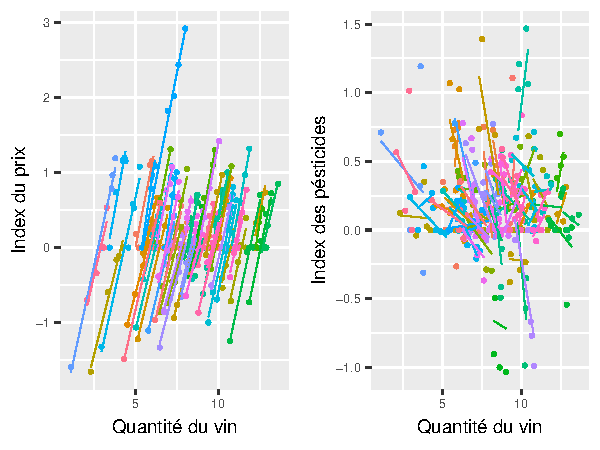
\includegraphics{Presentation_files/figure-beamer/unnamed-chunk-12-1.pdf}

\end{frame}

\begin{frame}{Visualisatoin des interdependances}
\protect\hypertarget{visualisatoin-des-interdependances-1}{}

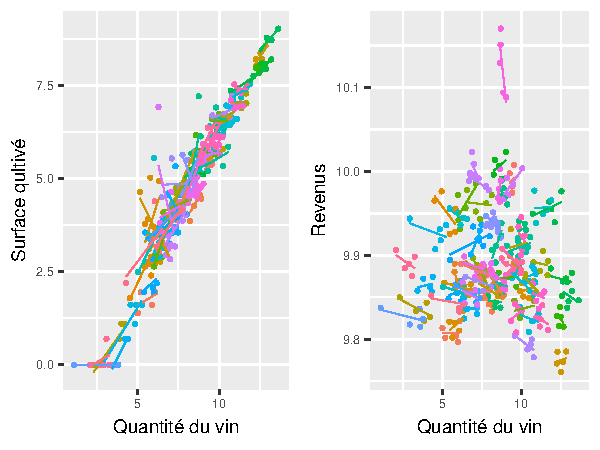
\includegraphics{Presentation_files/figure-beamer/unnamed-chunk-13-1.pdf}

\end{frame}

\begin{frame}{Random and fixed effects testing}
\protect\hypertarget{random-and-fixed-effects-testing}{}

\begin{itemize}
\tightlist
\item
  Poolability tests (tested versus pooled model)
\end{itemize}

\tiny
\begin{table}[!htbp] \centering
  \caption{Chow pooling test, p-values}
\begin{tabular}{@{\extracolsep{5pt}} l|cc} 
\\[-1.8ex]\hline 
\hline \\[-1.8ex] 
 & Random & Fixed \\ 
\hline \\[-1.8ex] 
Index prix & $0.535$ & $0.533$ \\ 
Index pesticides & $0.485$ & $0.451$ \\ 
Surface & $0$ & $0.0001$ \\ 
Revenus & $0.297$ & $0.247$ \\ 
\hline \\[-1.8ex]
\end{tabular} 
\end{table}

\end{frame}

\begin{frame}{Type of fixed effect testing}
\protect\hypertarget{type-of-fixed-effect-testing}{}

\begin{itemize}
\tightlist
\item
  Type of fixed effects testing
\end{itemize}

\tiny
\begin{table}[!htbp] \centering 
  \caption{Lagrange multiplier test, p-values}
\begin{tabular}{@{\extracolsep{5pt}} l|ccc} 
\\[-1.8ex]\hline 
\hline \\[-1.8ex] 
 & Individual & Time & Two-ways \\ 
\hline \\[-1.8ex] 
Index prix & $0$ & $0.169$ & $0$ \\ 
Index pesticides & $0$ & $0.222$ & $0$ \\ 
Surface & $0$ & $0.030$ & $0$ \\ 
Revenus & $0$ & $0.248$ & $0$ \\ 
\hline \\[-1.8ex] 
\end{tabular} 
\end{table}

\end{frame}

\begin{frame}{Correlation}
\protect\hypertarget{correlation}{}

\tiny
\begin{table}[!htbp] \centering
  \tiny\caption{Overall correlation}
\begin{tabular}{@{\extracolsep{5pt}} l|cccccc}
\\[-1.8ex]\hline
\hline \\[-1.8ex]
 & Quantité du vin & IP & Surface & Revenus & Index pésticides & Temps \\
\hline \\[-1.8ex]
Quantité du vin & $1$ & $0.154$ & $0.956$ & $-0.027$ & $-0.078$ & $-0.036$ \\      
IP & $0.154$ & $1$ & $0.045$ & $-0.037$ & $-0.127$ & $0.043$ \\
Surface & $0.956$ & $0.045$ & $1$ & $-0.057$ & $-0.060$ & $-0.064$ \\
Revenus & $-0.027$ & $-0.037$ & $-0.057$ & $1$ & $-0.052$ & $0.119$ \\
Index pésticides & $-0.078$ & $-0.127$ & $-0.060$ & $-0.052$ & $1$ & $0.291$ \\  
Temps & $-0.036$ & $0.043$ & $-0.064$ & $0.119$ & $0.291$ & $1$ \\
\hline \\[-1.8ex]
\end{tabular}
\end{table}

\tiny
\begin{table}[!htbp] \centering 
  \tiny\caption{Within transformation correlation}
\begin{tabular}{@{\extracolsep{5pt}} ccccccc} 
\\[-1.8ex]\hline 
\hline \\[-1.8ex] 
 & Quantité du vin & IP & Surface & Revenus & Index pésticides & Temps \\ 
\hline \\[-1.8ex] 
Quantité du vin & $1$ & $0.961$ & $0.366$ & $-0.160$ & $-0.228$ & $-0.199$ \\ 
IP & $0.961$ & $1$ & $0.289$ & $-0.009$ & $-0.127$ & $0.056$ \\ 
Surface & $0.366$ & $0.289$ & $1$ & $-0.166$ & $-0.191$ & $-0.310$ \\ 
Revenus & $-0.160$ & $-0.009$ & $-0.166$ & $1$ & $0.228$ & $0.652$ \\ 
Index pésticides & $-0.228$ & $-0.127$ & $-0.191$ & $0.228$ & $1$ & $0.414$ \\ 
Temps & $-0.199$ & $0.056$ & $-0.310$ & $0.652$ & $0.414$ & $1$ \\ 
\hline \\[-1.8ex] 
\end{tabular} 
\end{table}

\end{frame}

\begin{frame}{Within transformation results}
\protect\hypertarget{within-transformation-results}{}

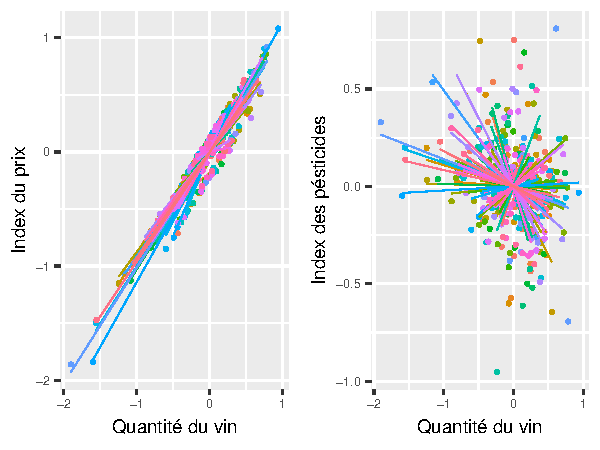
\includegraphics{Presentation_files/figure-beamer/unnamed-chunk-22-1.pdf}

\end{frame}

\begin{frame}{Within transformation results}
\protect\hypertarget{within-transformation-results-1}{}

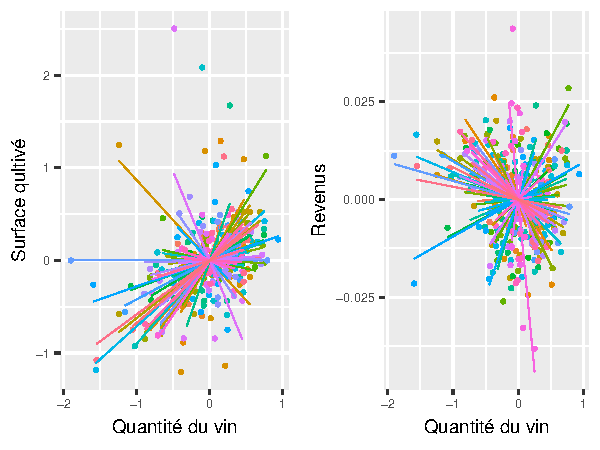
\includegraphics{Presentation_files/figure-beamer/unnamed-chunk-23-1.pdf}

\end{frame}

\begin{frame}{Modèlisation}
\protect\hypertarget{modelisation}{}

\begin{itemize}
\tightlist
\item
  Explication de la méthode utilisée

  \begin{itemize}
  \tightlist
  \item
    Panel data

    \begin{itemize}
    \tightlist
    \item
      Within transforation
    \item
      Fixed effects
    \item
      Obtained slopes are averages for all population
    \end{itemize}
  \item
    AIDS model

    \begin{itemize}
    \tightlist
    \item
      Interdependent equations (simultaneity bias)
    \item
      3SLS estimator (that is identical to ILS estimator)
    \item
      It generates consistent estimates
    \item
      The distribution of the estimators are normally distributed only
      in large samples
    \item
      The estimator is (asymptotically) efficient
    \end{itemize}
  \end{itemize}
\item
  Limites du modèle

  \begin{itemize}
  \tightlist
  \item
    Faible representation des effets hetérogenes entre les régions (nous
    estimons seulemnt les effets moyens)
  \item
    Les interferences induites par l'heterogénéité
  \end{itemize}
\end{itemize}

\end{frame}

\begin{frame}{Résultats d'estimation}
\protect\hypertarget{resultats-destimation}{}

\begin{itemize}
\tightlist
\item
  Les coefficients estimés avec leurs variance
\item
  Etude des erreurs
\item
  Vérification des hypothèses (5 hypothèses) :

  \begin{itemize}
  \tightlist
  \item
    La moyenne nulle des erreurs
  \item
    Homoscedacité
  \item
    Autocorrélation
  \item
    Spécification du modèle
  \item
    \ldots{} (à voir)
  \end{itemize}
\end{itemize}

\end{frame}

\begin{frame}{Les résultats OLS vs SUR}
\protect\hypertarget{les-resultats-ols-vs-sur}{}

\tiny

\begin{table}
\begin{center}
\begin{tabular}{l c c c }
\hline
 & OLS & WLS & SUR \\
\hline
Demande: ipi        & $0.93^{***}$  & $0.93^{***}$  & $0.93^{***}$  \\
                    & $(0.01)$      & $(0.01)$      & $(0.01)$      \\
Demande: ri         & $-5.75^{***}$ & $-5.75^{***}$ & $-2.00^{***}$ \\
                    & $(0.47)$      & $(0.47)$      & $(0.33)$      \\
Offre: ipi          & $0.90^{***}$  & $0.90^{***}$  & $0.92^{***}$  \\
                    & $(0.01)$      & $(0.01)$      & $(0.01)$      \\
Offre: si           & $0.08^{***}$  & $0.08^{***}$  & $0.02^{*}$    \\
                    & $(0.01)$      & $(0.01)$      & $(0.01)$      \\
Offre: iki          & $-0.17^{***}$ & $-0.17^{***}$ & $-0.05^{**}$  \\
                    & $(0.02)$      & $(0.02)$      & $(0.02)$      \\
\hline
Demande: R$^2$      & 0.95          & 0.95          & 0.94          \\
Offre: R$^2$        & 0.94          & 0.94          & 0.93          \\
Demande: Adj. R$^2$ & 0.95          & 0.95          & 0.94          \\
Offre: Adj. R$^2$   & 0.94          & 0.94          & 0.93          \\
Num. obs. (total)   & 690           & 690           & 690           \\
\hline
\multicolumn{4}{l}{\scriptsize{$^{***}p<0.001$, $^{**}p<0.01$, $^*p<0.05$}}
\end{tabular}
\caption{Statistical models}
\label{table : ols, wls and sur}
\end{center}
\end{table}
\tiny

\end{frame}

\begin{frame}{Disturbances correlation study}
\protect\hypertarget{disturbances-correlation-study}{}

\begin{itemize}
\tightlist
\item
  Les résidus sont non correlés avec les variables explicatives
\end{itemize}

\tiny
\begin{table}[!htbp] \centering 
  \caption{Errors correlation} 
  \label{} 
\begin{tabular}{@{\extracolsep{5pt}} ccccccc} 
\\[-1.8ex]\hline 
\hline \\[-1.8ex] 
 & OLS D & OLS O & WLS D & WLS O & SUR D & SUR O \\ 
\hline \\[-1.8ex] 
Vin & $0.232$ & $0.244$ & $0.232$ & $0.244$ & $0.273$ & $0.275$ \\ 
IP & $-0$ & $-0$ & $0$ & $-0$ & $0$ & $0$ \\ 
Surface & $0.271$ & $-0$ & $0.271$ & $0$ & $0.313$ & $0.236$ \\ 
Revenus & $0$ & $-0.480$ & $-0$ & $-0.480$ & $-0.393$ & $-0.542$ \\ 
Pesticides & $-0.308$ & $-0$ & $-0.308$ & $0$ & $-0.373$ & $-0.281$ \\
\hline \\[-1.8ex] 
\end{tabular} 
\end{table}

\end{frame}

\begin{frame}{Les résultats 2SLS, W2SLS et 3SLS}
\protect\hypertarget{les-resultats-2sls-w2sls-et-3sls}{}

\tiny

\begin{table}
\begin{center}
\begin{tabular}{l c c c }
\hline
 & 2SLS & W2SLS & 3SLS \\
\hline
Demande: ipi        & $1.19^{***}$  & $1.19^{***}$  & $1.19^{***}$  \\
                    & $(0.06)$      & $(0.06)$      & $(0.06)$      \\
Demande: ri         & $-5.67^{***}$ & $-5.67^{***}$ & $-5.67^{***}$ \\
                    & $(0.71)$      & $(0.71)$      & $(0.71)$      \\
Offre: ipi          & $-1.22$       & $-1.22$       & $-0.71$       \\
                    & $(1.97)$      & $(1.97)$      & $(1.96)$      \\
Offre: si           & $0.70$        & $0.70$        & $0.46$        \\
                    & $(0.59)$      & $(0.59)$      & $(0.58)$      \\
Offre: iki          & $-0.46$       & $-0.46$       & $-0.73^{*}$   \\
                    & $(0.34)$      & $(0.34)$      & $(0.32)$      \\
\hline
Demande: R$^2$      & 0.88          & 0.88          & 0.88          \\
Offre: R$^2$        & -3.37         & -3.37         & -1.60         \\
Demande: Adj. R$^2$ & 0.88          & 0.88          & 0.88          \\
Offre: Adj. R$^2$   & -3.40         & -3.40         & -1.62         \\
Num. obs. (total)   & 690           & 690           & 690           \\
\hline
\multicolumn{4}{l}{\scriptsize{$^{***}p<0.001$, $^{**}p<0.01$, $^*p<0.05$}}
\end{tabular}
\caption{Statistical models}
\label{table : 2sls, w2sls and 3sls}
\end{center}
\end{table}
\tiny

\end{frame}

\begin{frame}{Model choice tests}
\protect\hypertarget{model-choice-tests}{}

\begin{itemize}
\item
  Hausman 3SLS consistency test :

  Hausman specification test for consistency of the 3SLS estimation
\end{itemize}

data: dataWX Hausman = 5.5763, df = 5, p-value = 0.3497

\begin{itemize}
\tightlist
\item
  Likelihood test :
\end{itemize}

\tiny
\begin{table}[!htbp] \centering 
\begin{tabular}{@{\extracolsep{5pt}} cccccc} 
\\[-1.8ex]\hline 
\hline \\[-1.8ex] 
 & \#Df & LogLik & Df & Chisq & Pr(\textgreater Chisq) \\ 
\hline \\[-1.8ex] 
1 & $6$ & $-149.621$ & $$ & $$ & $$ \\ 
2 & $7$ & $-149.621$ & $1$ & $0$ & $1.000$ \\ 
3 & $8$ & $-65.614$ & $1$ & $168.013$ & $0$ \\ 
\hline \\[-1.8ex] 
\end{tabular} 
\end{table}

\end{frame}

\begin{frame}{Residuals tests}
\protect\hypertarget{residuals-tests}{}

\begin{itemize}
\tightlist
\item
  Residuals normality test
\end{itemize}

\tiny
\begin{table}[!htbp] \centering 
  \caption{Shapiro-Wilk test} 
\begin{tabular}{@{\extracolsep{5pt}} cccc} 
\\[-1.8ex]\hline 
\hline \\[-1.8ex] 
 & 2SLS & W2SLS & 3SLS \\ 
\hline \\[-1.8ex] 
Equation de demande & $0.00003$ & $0.00003$ & $0.00003$ \\ 
Equation d'offre & $0.00000$ & $0.00000$ & $0.00000$ \\ 
\hline \\[-1.8ex] 
\end{tabular} 
\end{table}

\normalsize

\begin{itemize}
\tightlist
\item
  Residuals heteroscedasticity test
\end{itemize}

\tiny 
\begin{table}[!htbp] \centering 
  \caption{Bartlett test}
\begin{tabular}{@{\extracolsep{5pt}} cccc} 
\\[-1.8ex]\hline 
\hline \\[-1.8ex] 
 & 2SLS & W2SLS & 3SLS \\ 
\hline \\[-1.8ex] 
Equation de demande & $0.975$ & $0.975$ & $0.975$ \\ 
Equation d'offre & $0.0003$ & $0.0003$ & $0.002$ \\ 
\hline \\[-1.8ex] 
\end{tabular}
\end{table}

\end{frame}

\begin{frame}{Residuals PDF visualisation}
\protect\hypertarget{residuals-pdf-visualisation}{}

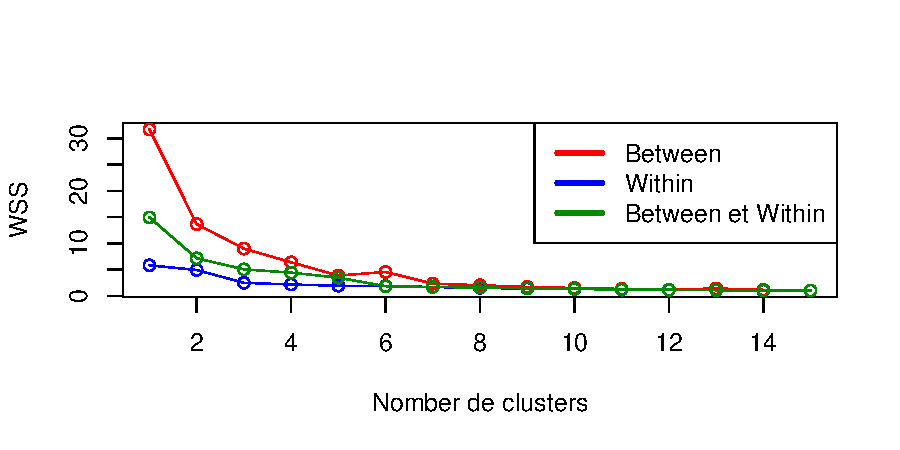
\includegraphics{Presentation_files/figure-beamer/unnamed-chunk-41-1.pdf}

\end{frame}

\begin{frame}{Residuals autocorrelation study for 3SLS}
\protect\hypertarget{residuals-autocorrelation-study-for-3sls}{}

\includegraphics{Presentation_files/figure-beamer/unnamed-chunk-42-1.pdf}

\end{frame}

\begin{frame}{Disturbances correlation study}
\protect\hypertarget{disturbances-correlation-study-1}{}

\begin{itemize}
\tightlist
\item
  Les résidus sont peux correlés avec les variables explicatives
\end{itemize}

\tiny
\begin{table}[!htbp] \centering 
  \caption{Errors correlation} 
\begin{tabular}{@{\extracolsep{5pt}} ccccccc} 
\\[-1.8ex]\hline 
\hline \\[-1.8ex] 
 & 2SLS D & 2SLS O & W2SLS D & W2SLS O & 3SLS D & 3SLS O \\ 
\hline \\[-1.8ex] 
Vin & $-0.561$ & $0.906$ & $-0.561$ & $0.906$ & $-0.561$ & $0.898$ \\ 
IP & $-0.746$ & $0.948$ & $-0.746$ & $0.948$ & $-0.746$ & $0.938$ \\ 
Surface & $-0.034$ & $0$ & $-0.034$ & $0$ & $-0.034$ & $0.032$ \\ 
Revenus & $0$ & $0$ & $0$ & $0$ & $-0$ & $0$ \\ 
Pesticides & $-0.113$ & $0$ & $-0.113$ & $0$ & $-0.113$ & $0.105$ \\ 
\hline \\[-1.8ex] 
\end{tabular} 
\end{table}

\end{frame}

\begin{frame}{Conclusions}
\protect\hypertarget{conclusions}{}

\begin{itemize}
\tightlist
\item
  Le rôle des pésticides
\item
  Le marché du vin
\item
  Validité
\item
  Limitations
\item
  Ouverture
\end{itemize}

\end{frame}

\begin{frame}{Bibliographie}
\protect\hypertarget{bibliographie}{}

\begin{itemize}
\tightlist
\item
  Cembalo L., Caracciolo F., \& Pomarici E. (2014). Drinking cheaply :
  the demand for basic wine in italy. \emph{Australian Journal of
  Agricultural and Resource Economics}, 58(3). 374-391.
\item
  Butault J-P., Delame N., Jacquet F. \& Zardet G. (2011). L'utilisation
  des pesticides en France: état des lieux et perspectives de réduction.
  \emph{Notes et études socio-économiques}, 35. 7-26
\item
  Pujol J. (2017). Apports des produits phytosanitaires en viticulture
  et climat : une analyse à partir des enquêtes pratiques culturales.
  \emph{Agreste Les Dossiers}. 39. 3-25
\end{itemize}

\end{frame}

\end{document}
